
% !TEX root = NotesDeCours.tex



\begin{frame}

  \color{bleu}

  \begin{flushleft}
    
    \Large
   	\bf
    
    Mécanique des fluides 	
    
  \end{flushleft}
  
  \ligne{3} % remplace: \noindent \thickline{0.5mm}{150}

  \begin{flushright}

    \rm

    \textrm{David} \textsc{Fabre}
    
    \vspace{3mm}
    
    IMFT / UPS
    
    Département de Mécanique
    
david.fabre@imft.fr

  \end{flushright}


  \begin{picture}(110, 30)(10, -20)
    \put(15, -17){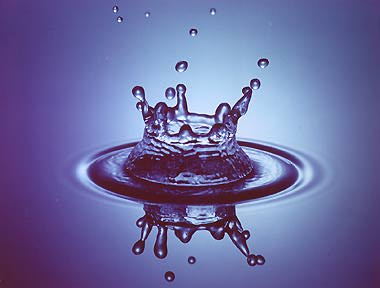
\includegraphics[height=42mm]{./Figures/splash.jpg}}
  \end{picture}

  \vspace{2mm}
  
  \begin{flushright}
    
    \Large
   	\bf
    
    0. Présentation et organisation du cours

  \end{flushright}


\end{frame}


%==================================================================================================
%\part{Présentation du cours}
%==================================================================================================




%--------------------------------------------------------------------------------------------------
\begin{frame}{Description du module}
%--------------------------------------------------------------------------------------------------

\small

\textbf{Format :} \medskip

\begin{itemize}
\item[\checkmark]
	24h Cours + 24h TD + 9h TP expérimentaux + 3h TP numériques
\item[\checkmark]
	Structuration du cours : 1 chapitre = 1 thème par semaine (2h) 
	\mytabbing{Structuration du cours :} avec 1 séance de TD associé (2h, la semaine d'après).
\item[\checkmark]
	Entre cours et TD : \textcolor{rouge}{exercice complémentaire} sur Moodle (travail personnel)
\item[\checkmark]
	TP expérimentaux et numériques : obligatoires, cf. informations sur le tableau d'affichage
\end{itemize}

\pause
\medskip

\textbf{Intervenants :} \medskip

\begin{itemize}
\item
	Cours : David FABRE (david.fabre@imft.fr)
\item
	TD : Mokhtar ZAGZOULE
\item
	TP expérimentaux : Frédéric MOULIN
\item
	TP numériques : David Fabre
	
\item ( Enseignants précédents : P. BRANCHER, P. LAURENS, S. SAINTLOS, F. CHARRU... )	
\end{itemize}

\pause
\medskip

\textbf{Evaluation :} \medskip

\begin{enumerate}
\item
	Première session : TP (20\%), examen partiel (30\%), examen terminal 1 (50\%)
\item 
	Seconde session : report de la note de TP (20\%), examen terminal 2 (80\%)
\end{enumerate}

\vspace{5mm}

\end{frame}
}

%--------------------------------------------------------------------------------------------------
\begin{frame}{Objectifs du cours}
%--------------------------------------------------------------------------------------------------

\small

\begin{itemize}
\item[\checkmark]
	Savoir analyser, décrire et caractériser les écoulements 
\item[\checkmark]
	Connaître les phénomènes physiques de base impliqués dans les écoulements
\item[\checkmark]
	Maîtriser la modélisation de ces mécanismes et leur mise en équation
\item[\checkmark]
	Savoir identifier les mécanismes dominants et ceux qui sont négligeables
\item[]
	$\rightarrow$ définition et exploitation des nombres sans dimension.
\item[\checkmark]
	Savoir simplifier les modèles en conséquence
\item[\checkmark]
	Maîtriser les techniques de résolution des équations régissant les écoulements 
\item[]
	$\rightarrow$ formulation complexe, analyse asymptotique, recherche de solutions auto-similaires, etc.
\end{itemize}

\bigskip

\hfill Remarque : liste non exhaustive\ldots

\vspace{20mm}

\end{frame}


%--------------------------------------------------------------------------------------------------
\begin{frame}{"Philosophie"}
%--------------------------------------------------------------------------------------------------

\small

Mécanique des fluides = discipline scientifique dont la maîtrise passe par la pratique régulière et
\mytabbing{Mécanique des fluides =} répétée des analyses et des techniques de modélisation et de résolution 
\mytabbing{Mécanique des fluides =} (exercices de TD, développements théoriques et démonstrations du cours)

\bigskip

\qquad $\rightarrow$ \textcolor{rouge}{travail personnel !} \quad (rappel : 1h de présentiel = 1h de travail perso)

\medskip
\qquad $\Rightarrow$ sur les 16 semaines du semestre = en moyenne 3h/semaine minimum (révisions incluses)

\vspace{5mm}
\pause

\textbf{Méthodologie}

\medskip
Entre le cours et le TD : \hfill (NB : pas de rappel de cours en TD\ldots)
\begin{enumerate}
\item relire le cours, 
\item refaire les démonstrations,
\item faire les exercices posés en cours,
\item travailler l'exercice complémentaire de la semaine.
\end{enumerate}

\vspace{5mm}
\pause

\textsl{Important} : rien n'est complètement trivial, il faut \textcolor{rouge}{se} poser des questions 
$\rightarrow$ \textcolor{rouge}{posez des questions !}

\medskip
Présupposé : il n'existe (presque) pas de question stupide en mécanique des fluides\ldots

\vspace{10mm}

\end{frame}

%--------------------------------------------------------------------------------------------------
\begin{frame}{Informations}
%--------------------------------------------------------------------------------------------------

\small

Quelques informations disponibles sur le tableau d'affichage du L3

\medskip

Plus d'informations sur la page Moodle du cours : \quad \texttt{\color{rouge} http://moodle.ups-tlse} 

\medskip

\qquad $\rightarrow$ puis taper dans \texttt{Recherche} : mécanique des fluides

\medskip

Clef d'accès : \texttt{\color{rouge} Reynolds}

\pause

\bigskip

Plusieurs documents pédagogiques ou administratifs mis en ligne :

\begin{itemize}
\item
	Syllabus du cours
\item
	Calendrier et protocole des examens
\item
	Résumés de cours
\item
	Compléments de cours
\item
	Enoncés de TD
\item
	\textcolor{rouge}{Exercices complémentaires} (énoncés et corrigés)
\item
	Enoncés et corrections d'autres exercices et problèmes 
\item
	Programmes informatiques
\item
 	 $[\ldots]$
\end{itemize}

\vspace{5mm}

\end{frame}


%--------------------------------------------------------------------------------------------------
\begin{frame}{Pré-requis et références bibliographiques}
%--------------------------------------------------------------------------------------------------

\small
\textbf{Pré-requis :} \smallskip

\begin{itemize}
\item
	Cours de \textcolor{rouge}{Mécanique des milieux continus} (MMC) du premier semestre
\item
	Cours de Thermodynamique du premier semestre
\item
	Notions de mécanique du point, des solides rigides et des systèmes.
\item
	Outils mathématiques : analyse, algèbre linéaire, géométrie différentielle, 
	\mytabbing{Outils mathématiques :} équations différentielles, intégrales multiples, \ldots
\end{itemize}

\pause

\medskip
\textbf{Modules "compagnons" du second semestre :} \smallskip

\begin{itemize}
\item
	Transferts thermiques 
\item
	Mécanique des solides 
\end{itemize}

\pause

\medskip
\textbf{Références :} \smallskip

\begin{itemize}
\item[] \hspace{-5mm}
	Guyon, Hulin \& Petit : \textsl{Hydrodynamique physique}.
		CNRS éditions, 2001.
\item[] \hspace{-5mm}
	Guyon, Hulin \& Petit : 
		\textsl{Ce que disent les fluides}.	Belin, 2005. 
\item[] \hspace{-5mm}
	Chassaing : \textsl{Mécanique des fluides : éléments d'un premier parcours}.
		Editions Cépaduès, 2000.
\item[] \hspace{-5mm}
	Ryhming : \textsl{Dynamique des fluides}.
		Presses Polytechniques et Universitaires Romandes, 2004.
\item[] \hspace{-5mm}
	Acheson : \textsl{Elementary Fluid Dynamics}. 
		Oxford University Press, 1990.
\end{itemize}

\end{frame}

%--------------------------------------------------------------------------------------------------
\begin{frame}{Plan du cours}
%--------------------------------------------------------------------------------------------------

\small

\begin{enumerate}
\item
  Introduction -- Analyse dimensionnelle
\item
  Forces dans les fluides au repos
\item 
  Forces dans les fluides en mouvement
\item
  Cinématique des écoulements
\item
  Equations de bilan
\item
  Ecoulements visqueux
\smallskip
\item[] \qquad $\rightarrow$ partiel
\smallskip
\item
  Ecoulements inertiels
\item
  Ecoulements potentiels
\item
  Ecoulements en conduite
\item
  Acoustique
\item
  Ecoulements compressibles
\item
  Ondes de choc
\smallskip
\item[] \qquad $\rightarrow$ examen terminal
\end{enumerate}

\vspace{5mm}

\end{frame}


